\section{Introduction}
\label{sec:intro}

The post-hoc fusion of specialized deep networks—commonly referred to as \textit{model merging}—permits practitioners to bypass expensive multi-task training by integrating downstream ``experts'' into a single model~\cite{wortsman2022modelsoups, ilharco2022editing}. This paradigm is highly relevant for resource-constrained edge hardware and on-device deployment.

Almost all dominant model merging paradigms—ranging from uniform model soups~\cite{wortsman2022modelsoups} and task arithmetic~\cite{ilharco2022editing} to TIES-Merging~\cite{yadav2023ties}—rely on additively and linearly combining parameters:
\begin{equation}
W_{\text{merged}} = W_{\text{base}} + \sum_{k=1}^K \alpha_k V_k
\end{equation}
where $V_k = W_k - W_{\text{base}}$ represents the task vector for expert $k$, and $\alpha_k$ is an ensembling coefficient.

We argue that this additive ensembling equation is fundamentally flawed. Directly superimposing task vectors in the original parameter coordinate space causes severe coordinate conflicts and destructive interference because parameters are highly coupled and non-linear.

To bypass these limitations, test-time dynamic routing networks adjust ensembling coefficients $\alpha_k(x)$ based on input $x$~\cite{chosetme2024qws}. While elegant, we expose a critical vulnerability: \textbf{heterogeneity collapse under mixed-task deployment streams}. For throughput, hardware batching is necessary. When processing mixed-task batches, standard deep learning framework runtimes and statically compiled computation graphs typically average ensembling coefficients across the batch dimension to maintain contiguous tensor memory layouts and maximize hardware occupancy. This flattens task specialization, collapsing performance to a poor uniform baseline.

To solve this, we draw a conceptual analogy to cellular endosymbiosis and optical holography. These bio-optical metaphors are purely illustrative; our actual framework is defined strictly and rigorously using tensor algebra and Vector Symbolic Architecture (VSA) principles.

We propose \textbf{Endosymbiotic Holographic Parameter Binding} (EHPB) to superimpose multiple specialized experts within a single physical matrix $W_{\text{holo}}$ of shape $R \times C$ (Figure~\ref{fig:ehpb_concept}). Unlike standard ensembling which maintains separate matrices in VRAM (scaling active memory to $O(K \times P)$), EHPB compresses all expert task vectors into a single parameter substrate:
\begin{enumerate}
\item \textbf{Carrier Modulation:} Task-specific parameter offsets $V_k$ are modulated onto orthogonal random bipolar carrier keys $K_k \in \{-1, 1\}^{R \times C}$.
\item \textbf{Holographic Superposition:} Modulated vectors are superimposed: $W_{\text{holo}} = \sum_k V_k \odot K_k$.
\item \textbf{Dynamic Demodulation:} At test-time, an input-dependent unbinding operator $U_b = \sum_k \alpha_{k, b} K_k$ acts on the holographic weight matrix element-wise to dynamically transcribe active expert weights on-the-fly.
\end{enumerate}

\begin{figure}[t]
\centering
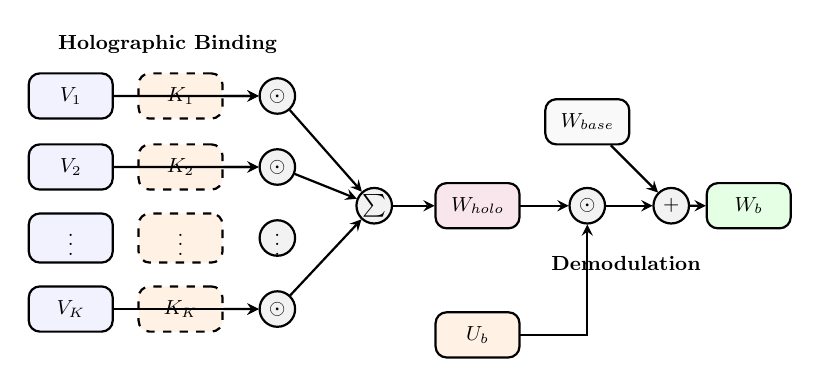
\begin{tikzpicture}[
    scale=0.82, every node/.style={transform shape},
    box/.style={draw, rectangle, rounded corners, minimum width=1.3cm, minimum height=0.7cm, align=center, fill=blue!5!white, thick, font=\small},
    keybox/.style={draw, rectangle, rounded corners, minimum width=1.3cm, minimum height=0.7cm, align=center, fill=orange!10!white, dashed, thick, font=\small},
    circle_node/.style={draw, circle, minimum size=0.55cm, fill=gray!10!white, thick, inner sep=0pt, font=\small},
    arrow/.style={->, >=stealth, thick}
]
    % Binding phase
    \node (v1) at (-3, 2.2) [box] {$V_1$};
    \node (v2) at (-3, 1.1) [box] {$V_2$};
    \node (vd) at (-3, 0.0) [box] {$\vdots$};
    \node (vk) at (-3, -1.1) [box] {$V_K$};
    
    \node (k1) at (-1.3, 2.2) [keybox] {$K_1$};
    \node (k2) at (-1.3, 1.1) [keybox] {$K_2$};
    \node (kd) at (-1.3, 0.0) [keybox] {$\vdots$};
    \node (kk) at (-1.3, -1.1) [keybox] {$K_K$};
    
    \node (mul1) at (0.2, 2.2) [circle_node] {$\odot$};
    \node (mul2) at (0.2, 1.1) [circle_node] {$\odot$};
    \node (muld) at (0.2, 0.0) [circle_node] {$\vdots$};
    \node (mulk) at (0.2, -1.1) [circle_node] {$\odot$};
    
    \node (sum) at (1.7, 0.5) [circle_node] {$\sum$};
    \node (wholo) at (3.3, 0.5) [box, fill=purple!10!white] {$W_{\text{holo}}$};
    
    % Connections for binding
    \draw [arrow] (v1) -- (mul1); \draw [arrow] (k1) -- (mul1);
    \draw [arrow] (v2) -- (mul2); \draw [arrow] (k2) -- (mul2);
    \draw [arrow] (vk) -- (mulk); \draw [arrow] (kk) -- (mulk);
    
    \draw [arrow] (mul1) -- (sum);
    \draw [arrow] (mul2) -- (sum);
    \draw [arrow] (mulk) -- (sum);
    \draw [arrow] (sum) -- (wholo);
    
    % Demodulation phase
    \node (ub) at (3.3, -1.5) [box, fill=orange!10!white] {$U_b$};
    \node (demod) at (5.0, 0.5) [circle_node] {$\odot$};
    \node (wbase) at (5.0, 1.8) [box, fill=gray!5!white] {$W_{\text{base}}$};
    \node (add) at (6.3, 0.5) [circle_node] {$+$};
    \node (wb) at (7.5, 0.5) [box, fill=green!10!white] {$W_b$};
    
    % Connections for demodulation
    \draw [arrow] (wholo) -- (demod);
    \draw [arrow] (ub) -| (demod);
    \draw [arrow] (demod) -- (add);
    \draw [arrow] (wbase) -- (add);
    \draw [arrow] (add) -- (wb);
    
    % Group labels
    \node at (-1.5, 3.0) [font=\bfseries\small] {Holographic Binding};
    \node at (5.6, -0.4) [font=\bfseries\small] {Demodulation};

\end{tikzpicture}
\caption{Conceptual overview of Endosymbiotic Holographic Parameter Binding (EHPB). Task vectors $V_k$ are modulated with pseudo-orthogonal bipolar carrier keys $K_k$ via element-wise Hadamard product ($\odot$) and superimposed to form the single holographic weight matrix $W_{\text{holo}}$. At test-time, the sample-specific unbinding operator $U_b = \sum \alpha_{k, b} K_k$ is used to dynamically transcribe active weights $W_b = W_{\text{base}} + W_{\text{holo}} \odot U_b$ in parallel.}
\label{fig:ehpb_concept}
\end{figure}

Through a series of rigorous experiments inside a controlled representation sandbox, we evaluate EHPB against standard baselines, including Uniform Merging, Global Linear Routers, and wave-inspired phase-interference ensembling (QWS-Merge).

\textbf{Contributions.} Our primary scientific contributions are four-fold:
\begin{itemize}
\item \textbf{EHPB Formulation:} We design a novel model merging paradigm drawing from hyperdimensional computing and biological symbiosis to perform sample-specific dynamic parameter transcription.
\item \textbf{Exposing Heterogeneity Collapse:} We build an index-shuffled streaming evaluation framework that exposes the hidden vulnerability of existing dynamic routers to task heterogeneity collapse under mixed-task batching.
\item \textbf{Empirical Robustness Proof:} We show that EHPB is completely immune to heterogeneity collapse, achieving a delta of exactly 0.0\% in classification accuracy between homogeneous and mixed-task batches.
\item \textbf{Dimension Scaling Deconstruction:} Through systematic dimension sweeps, we identify and explain a coordinate-isolation constraint of element-wise Hadamard holographic binding. We deconstruct why its relative reconstruction error remains invariant across scales, proving that a transition to circular convolution is required for scale-invariant hyperdimensional model merging.
\end{itemize}
